\documentclass[12pt]{article}
\usepackage{url, graphicx}
\usepackage{geometry}

 \geometry{
 a4paper,
 total={170mm,257mm},
 left=20mm,
 top=20mm,
 }

\title{\huge Lecture 1}
\author{Yutong Yan}
\date{}

\begin{document}
\maketitle

\section{The Central Paradigm of Computer Science}
\renewcommand{\labelitemii}{$\circ$}
\renewcommand{\labelitemiii}{$\cdot$}
\begin{itemize}
\item The central \textbf{\textit{paradigm}}  in computer science is that an algorithm \textbf{\textit{A}} is good if:
	\begin{itemize}
	\item \textbf{\textit{A}} runs in \textbf{\textit{polynomial time}} in the input size n.
	\item That is, \textbf{\textit{A}} runs in time $T$(n) = $O$($n^k$) for some constant number k.
		\begin{itemize}
		\item $T$(n) = 100n + 55
		\item $T$(n) = \( \frac{1}{2} \)$n^2$ + $999\log{}n$
		\item $T$(n) = 6$n^7$ + 900000$n^2$ - $\sqrt{n}$			
		\end{itemize}
	\item An algorithm is \textbf{\textit{bad}} if it runs in exponential time.
		\begin{itemize}
		\item $T$(n) = $2^n$ + 100$n^5$
		\item $T$(n) = $1.000000001^n$ - $n^3$ - n 
		\end{itemize}	
	\item An algorithm is \textbf{\textit{good}} if it runs in \textbf{\textit{polynomial time}} in the input size n.
	\begin{center}
	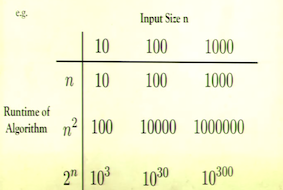
\includegraphics{lecture1a}
	\end{center}
	\end{itemize}
\end{itemize}


\section{Good versus Bad (Algorithms)}
\renewcommand{\labelitemii}{$\circ$}
\renewcommand{\labelitemiii}{$\cdot$}
\begin{itemize}
\item For example, consider the problem of sorting n numbers.
	\begin{itemize}
	\item A Good Algorithm: \textbf{MergeSort} runs in time $O$($n \cdot log{}n$)
	\item A Bad Algorithm: \textbf{BruteForce Search} runs in time $O$($n \cdot n!$) \(\gg\) $2^n$
	\end{itemize}
\end{itemize}


\section{An Equivalent Characterization}
\renewcommand{\labelitemii}{$\circ$}
\renewcommand{\labelitemiii}{$\cdot$}
\renewcommand{\labelitemiii}{$\rightarrow$}
\begin{itemize}
\item This central \textbf{\textit{paradigm}} has an equivalent formulation
	\begin{itemize}
	\item \textbf{\textit{A}} runs in \textbf{\textit{polynomial time}} in the input size n.
	\item The input sizes that \textbf{\textit{A}} can solve, in a fixed amount $T$ of time, \textbf{\textit{scales multiplicatively}} with increasing computational power.
	\begin{center}
	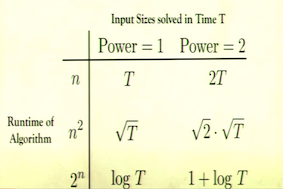
\includegraphics{lecture1b}
	\bigbreak
	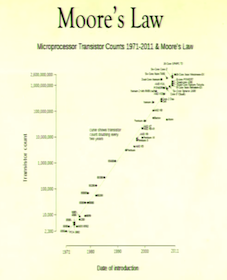
\includegraphics{lecture1c}
	\end{center}
	\item Moore's Law: Computational power \textit{doubles} roughly every two years.
		\begin{itemize}
		\item Functional time algorithms will never be able to solve large problems.
		\end{itemize}
	\end{itemize}

\clearpage	
\item The practical implications are perhaps simpler to understand with this \underline{latter} formulation.
\item Thus, improvements in hardware will \textit{never} overcome \textbf{\textit{bad algorithm design}}.
\item Indeed, the current dramatic breakthroughs in computer science are based upon batter (faster and higher performance) algorithmic techniques.
\end{itemize}


\section{Robustness}
\renewcommand{\labelitemii}{$\circ$}
\renewcommand{\labelitemiii}{$\cdot$}
\renewcommand{\labelitemiii}{$\rightarrow$}
\begin{itemize}
\item This measure of quality or "goodness" is \textbf{\textit{robust}}
	\begin{center}
	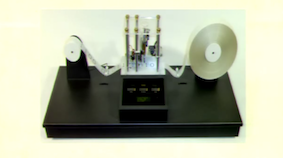
\includegraphics{lecture1d}
	\end{center}
\item All reasonable models of algorithms are polynomial time equivalent.
	\begin{itemize}
	\item Otherwise one model could perform, say, an exponential number of operations in the time another model took to perform just one.
	\end{itemize}
\item The standard formal model is the \textbf{Turing Machine}.
\end{itemize}









\section{Cryptography}



















\end{document}